\head{Октябрь}{Листок 9. Комбинаторика -- 2. Уровень 1.}

\epigraph{\textit{Как-то у Насреддина спросили, сколько на небе звёзд. Он ответил:
\\
— Этот вопрос меня интересует с давних пор. Но я думаю, что решить его можно только в том случае, если самому подняться на небо и сосчитать звёзды. Однако тут возникают два препятствия: если начать эту работу днём, то боюсь, что множество дел и толпы зевак помешают мне. Остаётся только подняться ночью на небо и заняться подсчётом звезд. Но это тоже опасно, потому что я не знаю, смогу ли найти на небе свечи или лампу, а в ночной темноте подсчитывать звёзды невозможно. Вот эти два препятствия и мешают мне решить вопрос о количестве звёзд на небе.}}{\textit{«Притчи о Насреддине»}}

В прошлом году мы занимались подсчётом различных вариантов выполнить что-либо. Например, мы выясняли, сколькими способами можно расставить в ряд $k$ из $n$ предметов. В литературе одна такая выборка называется \textit{размещением} и обозначается $A^k_n$. Если мы выбираем все предметы, то получаем перестановку. Число перестановок обозначается $A_n$ или $P_n$. Мы доказывали, что $P_n = n$! Когда мы говорим о размещениях, то для нас имеет значение порядок, в котором мы выбираем предметы. Если же требуется выяснить лишь сколько различных наборов из $k$ элементов можно выбрать из данного множества, то любой такой набор называется сочетанием, а число сочетаний, т.е. количество различных наборов из $k$ элементов, которые можно выбрать из имеющихся $n$, обозначается $C^n_k$. 
\\
В частности справедлива формула \boxed{P_k \cdot C^k_n = A^k_n}

\section{Посчитаем варианты, или «шары и перегородки».}

\epigraph{\textit{-- Чем займёмся, уважаемые кроты?
\\
-- А почему бы нам не посчитать?}}{\textit{Из мультфильма «Дюймовочка»}}

\begin{figure}[H]
\begin{minipage}{0.75\linewidth}\setlength{\parindent}{1.5em}
    \begin{thm}
        Сколькими способами можно разбить наш класс на две (необязательно равные) команды?
    \end{thm}
    \begin{thm}
        У Эрика есть 20 друзей и каждый день он приглашает некоторых из них в гости так, чтобы компания ни разу не повторялась (в какой-то день он может не пригласить никого). Сколько дней он сможет так делать?
    \end{thm}
    \begin{ques}
        Что общего между двумя предыдущими задачами?
    \end{ques}
\end{minipage}
\hfill
\begin{minipage}{0.2\linewidth}
    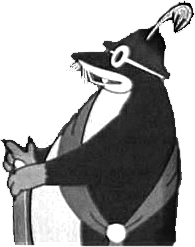
\includegraphics[width=0.95\columnwidth]{img/9.0.1 krot.png}
\end{minipage}
\end{figure} 

\begin{thm}
    Сколькими способами можно разложить 2009 конфет в 17 коробок так, чтобы в каждой коробке была хотя бы одна конфета? (Конфеты считать одинаковыми, коробки разными)
    \par
    \textit{\textbf{Ответ.}} $C^{16}_{2008} = \dfrac{2008 \cdot 2007 \cdot ... \cdot 1993}{16!}$
    \par
    \textit{\textbf{Решение.}} Разложим все 2009 конфет в ряд и будем расставлять между ними перегородки. Поскольку коробок 17, то перегородок потребуется 16. Все, что будет ДО первой перегородки, положим в первую коробку, от 1 до 2 – во вторую коробку, от 2 до 3 – в третью и так далее, всё, что ПОСЛЕ шестнадцатой перегородки – положим в семнадцатую коробку. Таким образом, задача свелась к подсчёту количества способов выбрать 16 промежутков (для перегородок) из 2009 возможных (между 2009-ю конфетами 2008 промежутков), а это $C^{16}_{2008}$ или $\dfrac{2008 \cdot 2007 \cdot ... \cdot 1993}{16!}$
\end{thm}

\begin{thm}
    Вета, Рая и Женя купили 40 одинаковых шоколадок. Сколькими различными способами они могут разделить эти шоколадки (не ломая) между собой?
    \par
    \textit{\textbf{Решение.}} Добавим к уже имеющимся шоколадкам два леденца и сосчитаем все возможные способы расположения в ряд этих 42 сладостей. Понятно, что всего существует $C^2_{42}$ таких способов, т.к. порядок зависит только от расположения леденцов, а два леденца можно расположить на 42 местах $C^2_{42}$ способами. Каждому такому способу соответствует свой раздел сластей: отдадим Вете все шоколадки до первого леденца (если этот леденец первый, то не дадим ничего), Рае – от первого до второго, а Жене – все шоколадки после второго леденца. Таким образом, 
    \par
    \textit{\textbf{Ответ}}: $C^2_{42}$ способов.
\end{thm}

\begin{thm}
    Андрей, Гоша и Рома ходили в лес за грибами. Всего они нашли 15 подосиновиков, 10 подберезовиков и 5 мухоморов. Сколькими способами они могут разделить эти грибы между собой? (грибы резать нельзя, необязательно грибы должны быть у каждого, грибы одного сорта считаются неразличимыми.
\end{thm}

\begin{thm}
    Лида, Ира и Ксюша тоже ходили в лес за грибами. Ира собирала только подосиновики, Ксюша – только подберезовики, а Лида – только мухоморы. Всего они нашли 30 грибов. Сколько различных вариантов наборов грибов может быть?
\end{thm}

\begin{thm}
    Батарейка за работу в классе поставила 17 «плюсиков». Сколькими способами она это могла сделать, если в классе 22 человека?
\end{thm}



\begin{thm}
    Чемпионат класса по шахматам проводился в один круг. Сколько было сыграно партий, если в турнире участвовало 17 человек?
\end{thm}

\begin{thm}
    Сколько есть способов расставить 8 ладей не бьющих друг друга на шахматную доску?
\end{thm}

\begin{thm}
    Сколькими способами можно разбить 20 человек на пары? А $2n$ человек?
\end{thm}

\begin{thm}
    На танцплощадке собрались 10 юношей и 10 девушек. Сколькими способами они могут разбиться на пары для участия в следующем танце? А если девушек и юношей $n$?
\end{thm}

\begin{thm}
    Сколько существует 7-мизначных чисел, сумма цифр которых четна?
\end{thm}

\begin{thm}
    Сколько существует 9-тизначных чисел, в которых одинаковы хотя бы 2 цифры?
\end{thm}

\begin{thm} $^*$
    Для какого $n > 1$ количество $n$--значных чисел, у которых есть одинаковые цифры больше количества $n$--значных чисел с разными цифрами?
\end{thm}

% Мы уже говорили о числе размещений и числе сочетаний $n$ предметов, $A^k_n$ и $C^k_n$. Вспомните, в чём разница между этими понятиями и по каким формулам их можно вычислить. О свойствах чисел сочетаний и их связи с треугольником Паскаля мы также уже говорили. Далее приведено несколько несложных задач, в которых используются эти свойства.

\begin{ex}
    У Руслана есть 7 книг по химии, а у Миши – 8 книг по физике. Сколькими способами они могут обменять три книги одного на три книги другого?
\end{ex}

\begin{ex}
    Сколькими способами можно разбить класс из 22 человек на две футбольные команды по 11 человек в каждой?
\end{ex}

\begin{ex}
    На плоскости отмечено 10 точек так, что никакие три из них не лежат на одной прямой. Сколько существует треугольников с вершинами в этих точках?
\end{ex}

\begin{ex}
    На прямой отмечено 10 точек, а на параллельной ей прямой – 11 точек. Сколько существует а) треугольников; б) четырёхугольников с вершинами в этих точках?
\end{ex}

\begin{ex}
    Сколькими способами можно разбить число 11 на три ненулевых слагаемых? (Способы, отличающиеся порядком слагаемых, считаются различными.)
\end{ex}

\begin{ex}
    Сколькими способами можно разложить 12 монет по 5 кошелькам, чтобы ни один не был пуст? (Класть один кошелёк в другой не разрешается)
\end{ex}

\centerline{\textit{\textbf{Лирическое отступление.}}}

Как-то в один из ресторанов некого испанского города пришли 9 студентов. Они только что успешно сдали экзамены и решили отметить сие радостное событие. Однако в ресторане они долго спорили, кто и где должен сидеть за столом, и подняли такой невероятный шум, что хозяин ресторана не выдержал и сказал: ''Да садитесь сегодня как угодно! Вы можете приходить ко мне все вместе каждый день и обедать, рассаживаясь каждый день по--новому. Как только вы сядете так, как вы уже ранее садились, с того дня я буду кормить вас бесплатно!'' Шум был устранён, но, как вы думаете, не погорячился ли хозяин? Как быстро наступит день, когда студенты придут к нему за бесплатным обедом?